\documentclass{article}
\usepackage[utf8]{inputenc}
\usepackage[T1]{fontenc}
\usepackage[ngerman]{babel}
\usepackage{xcookybooky}
\begin{document}

\setHeadlines
{%  fuer den Fall das ngerman geladen wurde
    inghead = Zutaten,
    prephead = Zubereitung,
    hinthead = Tipp,
    portionvalue = Portionen,
}

\setRecipeLengths{
    preparationwidth = 0.7\textwidth,
    ingredientswidth = 0.4 \textwidth,
}

% Sophie
\begin{recipe}
[ % Optionale Eingaben
%    preparationtime = {\unit[30]{min}},
%    bakingtime={\unit[10]{min}},
%   bakingtemperature={\Fanoven\ \unit[250]{C}},
%    portion = \portion{4},
    %calory,
    source = Sophie
]
{Französische Zwiebelsuppe}

\graph{
    big = sophie/Zwiebelsuppe.png,
}

\ingredients[8]
{% Zutatenliste
    \unit[300]{g} & Zwiebeln \\
    2 & Knoblauchzehen \\
    \unit[1]{EL} & Butterschmalz \\
    \unit[1]{EL} & Mehl \\
    \unit[1 \nicefrac{1}{4}]{L} & Brühe \\
     & Salz und Pfeffer  \\
     4 & Brotscheiben  \\
     \unit[100]{g} & Geriebener Käse
}

\preparation
{ % Schrittweise Zubereitung
    \\
Die Zwiebeln in Ringe schneiden, Knoblauch fein hacken. Butterschmalz in einem Kochtopf zerlassen, Zwiebeln und Knoblauch dazugeben und goldgelb rösten.

1 EL Mehl hinzugeben und unter Rühren für ca. 5 Minuten durchschwitzen. Langsam mit der Brühe aufgießen und ca. 20-25 Minuten aufkochen lassen. Kräftig mit Salz und Pfeffer würzen.

Das Brot würfeln und rösten. Die Suppe in feuerfeste Tassen füllen, die Brotwürfel dazugeben und mit Käse überstreuen. Im vorgeheizten Backofen bei 250 °C für 10 Minuten backen.

}

\hint
    {% Hinweise
    Geht auch ohne das Überbacken, aber Käse macht einfach viele Dinge besser.

    Das Bild ist aus dem Internet geklaut, aber selbst gemacht sieht genauso aus!
    }

\end{recipe}

\newpage
%\begin{recipe}
[ % Optionale Eingaben
%    preparationtime = {\unit[30]{min}},
    bakingtime={\unit[30]{min}},
    bakingtemperature={\Fanoven\ \unit[200]{C}},
   portion = \portion{4},
    %calory,
    source = Sophie
]
{Quiche Lorraine}

\introduction{
    \# Rezept meiner Mutter, bisher unübertroffen von allem, was meine französischen Freundinnen gebacken haben.
}

\graph{
    big = sophie/Quiche,
}

\ingredients[11]
{% Zutatenliste
    \unit[200]{g} & Mehl \\
    \unit[100]{g} & Butter \\
    \unit[\nicefrac{1}{2}]{TL} & Salz \\
     & Beliebige Dinge für die Füllung (s. Tipp) \\
    4 & Eier \\
    \unit[\nicefrac{1}{4}]{L} & Sahne \\
    \unit[125]{g} & Geriebener Käse \\
    \unit[\nicefrac{1}{2}]{TL} & Weißer Pfeffer \\
    \unit[\nicefrac{1}{2}]{TL} & Salz
}

\preparation
{ % Schrittweise Zubereitung
    \\
Für den Teig Mehl, Salz und Butter in Flocken mit 5 EL Wasser rasch zu einem geschmeidigen Teig verarbeiten. In Pergamentpapier einschlagen und in den Kühlschrank stellen

Den Backofen auf 200 °C vorheizen. Eine Springform mit Butter ausstreichen und mit Mehl bestäuben. Den Teig ausrollen und so in die Springform legen, dass der Teig einen Rand bildet. 

Den Teig für ca. 10 Minuten vorbacken (es hilft, den Teig mit trockenen Bohnen auf Pergamentpapier zu beschweren, damit die Seiten nicht einfallen).

Für die Füllung die Eier trennen. Die Eigelbe mit Sahne, Salz, Pfeffer und eventuellen anderen Gewürzen (z.B. Muskat) verquirlen. Den Käse und die sonstige Füllung (Gemüse o.ä.) unterziehen. Die Eiweiße mit etwas Salz steif schlagen und unter die Eigelbmasse heben. 

Die Füllung auf den vorgebackenen Teig geben und die Quiche für mindestens 30 Minuten im Backofen bei 200 °C backen.
}

\hint
    {% Hinweise
    Für die Füllung: Klassischerweise Speck/Schinken (200 g), ansonsten z.B. gedünstetes Gemüse (mediterran mit Paprika, Zucchini und getrockneten Tomaten ; oder Lauch mit Karotten). Ich mag die Kombination Spinat + Schafskäse sehr gerne.
    
    Meine französischen Freund:innen haben das Trennen der Eier meist weggelassen, um Zeit zu sparen. Ich finde, die Quiche wird durch den Eischnee aber sehr viel fluffiger und insgesamt leckerer.

    Ich sollte häufiger fotografieren, was ich koche/backe. Weil ich das nicht getan habe hier ein Internet-Foto zur Inspiration.
    }

\end{recipe}

%\newpage
%\begin{recipe}
[ % Optionale Eingaben
%    preparationtime = {\unit[30]{min}},
    bakingtime={\unit[50]{min}},
    bakingtemperature={\Fanoven\ \unit[180]{C}},
    %calory,
    source = Sophie
]
{Zitronen-Meringue-Tarte}

\introduction{
    \# Rezept meiner französischen Mitbewohnerin. Sie hat gerne die geniale Aufteilung der getrennten Eier in den verschiedenen Tarte-Komponenten betont.
}

\graph{
    big = sophie/Zitronentarte,
}

    \ingredients[19]
{% Zutatenliste
    \textit{Mürbteig} & \\%evtl anzupassen
    \unit[250]{g} & Mehl \\
    \unit[125]{g} & Butter \\
    \unit[70]{g} & Zucker \\
    2 & Eigelbe \\
    ca. \unit[50]{mL} & Wasser \\
    \unit[1]{Prise} & Salz \\
    \textit{Zitronencreme} & \\%evtl anzupassen
    2 & Bio-Zitronen \\
    \unit[180]{g} & Zucker \\
    2 & Eier \\
    2 & Eigelbe \\
    \unit[200]{mL} & Saure Sahne \\
    \unit[1]{Prise} & Salz \\
    \textit{Meringue-Haube} & \\%evtl anzupassen
    4 & Eiweiße \\
    \unit[150]{g} & Puderzucker \\
    \unit[1]{Prise} & Salz
}

\preparation
{ % Schrittweise Zubereitung
    \\
Den Teig vorbereiten: Den Ofen auf 180 °C (Umluft) vorheizen. Die Eigelbe und Zucker mit etwas Wasser verquirlen. Mehl und Butter mit den Fingern mit den Fingern leicht zusammenkneten, bis eine sandartige Konsistenz erreicht wird. Die flüssige Mischung zu Mehl und Butter geben und den Teig zu einem Ball kneten. Den Teig dann ausrollen, in die Springform legen und den Teigboden einige Mal mit einer Gabel anstechen. Für 10 Minuten backen (den Teig mit Bohnen beschweren ; der Teig sollte durch das Backen nicht braun werden oder nur leicht).

Die Creme zubereiten: Zwei Eier mit zwei weiteren Eiweißen, der sauren Sahne und dem Zucker verrühren. Den Saft von zwei Zitronen und deren abgeriebene Schale dazugeben. Den Teig aus dem Ofen holen und die Bohnen entfernen, dann die Creme auf den Teig geben und für 30 Minuten backen.

In der Zwischenzeit die Meringue vorbereiten: Die vier verbleibenden Eiweiße mit einer Prise Salz steif schlagen. Dann den Puderzucker nach und nach unter Rühren zugeben, bis die gewünschte Konsistenz erreicht ist.

Wenn die Creme gestockt ist (evtl. etwas länger als 30 Minuten backen), die Meringue auf der Tarte verteilen und für weitere 10 Minuten backen, bis die Meringue leicht bräunlich wird. Für eine härtere Meringue sollte die Tarte weitere 30 Minuten im Ofen bleiben.

}

\hint
    {% Hinweise
    Klingt nach Arbeit, lohnt sich aber, versprochen!
    
    Der Zucker in allen drei Komponenten kann nach Belieben reduziert werden.
    }

\end{recipe}

%\newpage

% Chris

\begin{recipe}
[ % Optionale Eingaben
    preparationtime = {\unit[15]{min}},
    portion = \portion{4},
    source = Chris' Mitbewohner David
]
{Hirsesalat}

\introduction{
    \# High Protein 
    \# Flexibel Einsetzbar
    \# Macht sich gut bei jedem Grillbuffet
}

\graph{
    big = chris/Hirse
}

\ingredients
{% Zutatenliste
    \unit[250]{g} & Hirse \\
    \unit[250]{g} & Feta \\
    4 & Tomaten \\
    1 & Gurke \\
    1 & kl. Dose Mais \\
    1 & kl. Dose rote Bohnen \\
    & etwas Balsamico \\
}

\preparation
{ % Schrittweise Zubereitung
    \\
    Hirse mit dem doppelten Volumen Wasser in einen Topf geben.
    Einmal aufkochen und anschließend abgedeckt auf sehr niedriger Stufe köcheln lassen.
    Die Hirse ist fertig sobald das Wasser vollständig aufgenommen oder verdampft wurde. 
    In der Zwischenzeit das Gemüse und den Feta würfeln und die Dosen abgießen.
    Wenn die Hirse fetig ist, alles in einer großen Schüssel vermischen und mit Salz, Pfeffer und Balsamico Essig abschmecken.}

\hint
    {% Hinweise
    Falls du den Salat für mehrere Tage gekocht hast, gib den Balsamico immer nur an das was du direkt essen möchtest, die Tomaten werden sonst schneller schlecht. 
    Wenn du das berücksichtigst, hält sich der Salat aber problemlos für 3-4 Tage im Kühlschrank.
    }
\end{recipe}

\newpage
\input{./chris/Gnocci_mit_Gemüse.tex}
\newpage

\begin{recipe}
[ % Optionale Eingaben
    preparationtime = {\unit[5]{min}},
    portion = \portion{4},
    source = Chris' Oma
]
{Stippmilch}

\introduction{
    \# Münsterländer Original
    \# Schnell gemacht
    \# Mit dem extra an Calcium
}

\graph{
    small = chris/Stippmilch1,
    big = chris/Stippmilch2,
}

\ingredients
{% Zutatenliste
    \unit[500]{g} & Magerquark \\
    etwas & Milch (Kuh oder Hafer) \\
    etwas & Zucker (1-5 Esslöffel) \\
    & Toppings nach Belieben \\
}

\preparation
{ % Schrittweise Zubereitung
    \\
    Magerquark in einer Schüssel mit der Milch verrühren, sodass eine glatte Maße entsteht. 1-5 Esslöffel Zucker hinzugeben und verrühren. 
    Die Stippmilch kann mit frischem Obst, Schokostreußeln, Kakao, Fruchtsirup etc. gegessen werden.
    Meine Lieblingsvariante ist mit frischen Erdbeeren. }
\end{recipe}

\newpage

% Malte
\begin{recipe}
[ % Optionale Eingaben
    preparationtime = {\unit[20]{min}},
    bakingtime={\unit[20]{min}},
    bakingtemperature={\Fanoven\ \unit[180]{C}},
    %portion = \portion{8},
    %calory,
    source = Malte
]
{Pflaumen und Rosenkohl Häppchen}

\introduction{
    \# Lecker Verwicklung
}

\graph{
    small = malte/p1,
    big = malte/p2,
}

\ingredients
{% Zutatenliste
    & Gedörrte Pflaumen \\
    & Rosenkohl \\
    & Bacon \\
    & Honig \\
}

\preparation
{ % Schrittweise Zubereitung
    \\
    Rosenkohl würzen und mit je einem Streifen Bacon umwickeln.
    Dann mit etwas Honig bestreichen.
    Backen bis der Rosenkohl durchgegart ist.

    Pflaumen mit je einem Streifen Bacon umwickeln.
    Backen bis der Bacon gut gebräunt ist.

    Kann beides sowohl warm als auch kalt serviert werden.
}

\hint
    {% Hinweise
    Kann beides zur besseren Handhabung auch mit Holzspießchen fixiert werden.

    Grade von den Pflaumen etwas mehr machen, die gehen schnell weg.

    Die Bilder wurde von einer glücklichen KI generiert.
    }

\end{recipe}

\newpage

\begin{recipe}
[ % Optionale Eingaben
    preparationtime = {\unit[15]{min}},
    bakingtime={\unit[20]{min}},
    bakingtemperature={\Fanoven\ \unit[180]{C}},
    portion = \portion{4},
    %calory,
    source = Malte
]
{Rote Bete mit Feta und Cashews}

\introduction{
    \# Interessante Kombi
}

\graph{
    small = malte/b1,
    big = malte/b2,
}

\ingredients[7]
{% Zutatenliste
    \unit[500]{g} & Rote Bete \\
    2 & Rote Zwiebeln \\
    \unit[200]{g} & Feta- oder Ziegenkäse \\
    \unit[150]{g} & Cashewkerne \\
    \unit[3]{TL} & Honig \\
    \unit[2]{EL} & Öl
}

\preparation
{ % Schrittweise Zubereitung
    \\
    Rote Bete kochen und schälen oder gleich vorbereitete Kaufen.

    Rote Bete in größere Häppchen schneiden.
    Zwiebeln in große Stücke schneiden (\nicefrac{1}{8} oder so).
    Beides gemischt in eine Auflaufform verteilen, würzen und das Öl untermischen.

    Im Ofen bei \unit[180]{C} kurz für ca. 5min backen.

    Cashews zerkleinern und darüber streuen.
    Darauf den Honig verteilen.

    Wieder in den Backofen schieben, bis der Käse und die Cashews leicht braun werden.

    Zusammen mit einer Beilage wie Baguettes oder Reis servieren.
}

\hint
    {% Hinweise
    Kann auch sehr gut kalt gegessen werden.

    Die Bilder wurde von einer glücklichen KI generiert.
}

\end{recipe}

\newpage
\begin{recipe}
[ % Optionale Eingaben
    preparationtime = {\unit[20]{min}},
    bakingtime={\unit[6]{h}},
    %bakingtemperature={\Fanoven\ \unit[170]{C}},
    portion = \portion{8},
    %calory,
    source = Malte
]
{Kalte Himbeernachspeise}

\introduction{
    \# Kalte Kalorienbombe
}

\graph{
    small = malte/h1,
    big = malte/h2,
}

\ingredients
{% Zutatenliste
    \unit[500]{g} & Himbeeren, gerne auch gefroren \\
    \unit[200]{g} & Baiser Häubchen \\
    \unit[400]{ml} & Schlagsahne \\
    \unit[150]{g} & Joghurt \\
    2 Päckchen & Vanillezucker \\
    \unit[2]{cl} & Himbeergeist oder ein Äquivalent, zum Beispiel auch Sirup \\
}

\preparation
{ % Schrittweise Zubereitung
    \\
    Baiser zu Brocken zerkrümeln und als unterste Schicht in eine Schale streuen.
    Darüber 2 EL Himbeergeist und|oder Sirup gießen.
    Darauf die Himbeeren streuen.

    Schlagsahne mit Vanillezucker schlagen und den Joghurt unterheben.
    Die Mischung als letzte Schicht verteilen.

    Dann einen halben Tag im Kühlschrank durchziehen lassen.
    Wenn man will, kann man das ganze auch im Gefrierfach anfrieren lassen.
}

\hint
    {% Hinweise
    Vor dem Servieren mit Himbeeren oder Baiser verzieren.

    Die Bilder wurde von einer glücklichen KI generiert. Es ist vermutlich einfache alles in einer großen Schale zuzubereiten und nicht in vielen kleinen.
    }

\end{recipe}

\newpage

% Lynn

\begin{recipe}
[ % Optionale Eingaben
    preparationtime = {\unit[20]{min}},
    portion = \portion{2},
    %calory,
    source = Lynn
]
{Bauernsalat}

\introduction{
    \# Copyright das griechische Restaurant bei uns um die Ecke
}

\graph{
    small = lynn/salat1,
    big = lynn/salat2,
}

\ingredients
{% Zutatenliste
    2 & Tomaten \\
    \nicefrac{1}{2} & Gurke \\
    \unit[\nicefrac{1}{2}]{Glas} & Oliven \\
    1 & grüne Paprika \\
    1 & Feta \\
    1 & rote Zwiebel \\
    Etwas & Salat \\
    \unit[3]{Schluck} & weißer Balsamico \\
    \unit[Ein paar]{Schuss} & Olivenöl \\
    \unit[1]{TL} & Honig \\
    \unit[1]{TL} & Senf \\
    Etwas & Gewürze 
}

\preparation
{ % Schrittweise Zubereitung
    \\
    Die Tomaten, Gurke, Paprika und den Feta würfeln und zusammengeben. Oliven und Salat ebenfalls dazugeben. 
    
    Dressing aus Essig, Öl, Honig und Senf zusammenmischen. Mögliche Gewürze zum hinzufügen sind Pfeffer, Salz, Knoblauch oder beliebige Kräuter.
    
    Die Zwiebel in Ringe schneiden und oben auf den Salat geben.
}

\hint
    {% Hinweise
    Die Bilder sind zwar von einer KI, aber wenn dein Salat so bunt aussieht, dann hast du alles richtig gemacht.
    }

\end{recipe}

\newpage
\begin{recipe}
[ % Optionale Eingaben
    preparationtime = {\unit[30]{min}},
    bakingtime={\unit[15]{min}},
    bakingtemperature={\Fanoven\ \unit[250]{°C}},
    portion = \portion{2},
    %calory,
    source = Lynn
]
{Flammkuchen}

\introduction{
    \# Minimaler Einkaufsaufwand
}

\graph{
    small = lynn/flamm1,
    big = lynn/flamm2,
}

\ingredients
{% Zutatenliste
    \unit[250]{g} & Mehl \\
    \unit[125]{mL} & Wasser \\
    Etwas  & Salz \\
    \unit[3]{EL} & Öl \\
    \unit[125]{g} & Speck \\
    oder \\
    eine Hand voll & Champignons \\
    2 & rote Zwiebeln \\
    \unit[250]{g} & Créme Fraîche
}

\preparation
{ % Schrittweise Zubereitung
    \\
    Die Zutaten für den Teig zusammengeben und etwas kneten. In 2 Teile teilen und sehr dünn ausrollen. Auf 2 Blechen verteilen.
    
    Die Creme Fraiche auf dem Teig verteilen und mit Salz und Pfeffer würzen. Zwiebeln in Halbringe schneiden und mit einem Schluck Wasser 1 Minute bei ~500 W in Mikrowelle geben, damit die Zwiebeln im Ofen nicht so leicht anbrennen. 
    
    Zwiebeln und Speck oder Pilze (oder beides) verteilen und die Flammkuchen 15 Minuten bei 250 °C backen.
}

\hint
    {% Hinweise
    Die Erfahrung zeigt: Eine Person ist durchaus in der Lage ein Blech alleine zu essen…

    Alternative Belagmöglichkeiten sind: Tomaten, Oliven und Käse oder Zwiebeln, Feta und Honig.
    
    Auch diese Bilder sind von einer KI.
    }

\end{recipe}

\newpage
\begin{recipe}
[ % Optionale Eingaben
    preparationtime = {\unit[30]{min}},
    bakingtime={\unit[50]{min}},
    bakingtemperature={\Fanoven\ \unit[180]{°C}},
    portion = \portion{12},
    %calory,
    source = Lynn
]
{Käsekuchen}

\introduction{
    \# kein Käse enthalten
}

\graph{
    small = lynn/kuchen1,
    big = lynn/kuchen2,
}

\ingredients
{% Zutatenliste
    \unit[200]{g} & Mehl \\
    \unit[75]{g} & Zucker \\
    1 & Ei \\
    \unit[1]{TL} & Backpulver \\
    \unit[500]{g} & Quark \\
    2  & Eier \\
    \unit[140]{g} & Zucker \\
    \unit[1]{Pck.} & Vanillepudding \\
    \unit[100]{g} & Saure Sahne \\
    \unit[80]{mL} & Öl \\
    \unit[240]{mL} & Milch \\
    \unit[1]{Dose} & Mandarinen \\
    \unit[1]{Pck.} & Tortenguss 
}

\preparation
{ % Schrittweise Zubereitung
    \\
    Für den Teig Mehl, 75\,g Zucker, ein Ei und Backpulver mit dem Rührer mixen und auf dem Boden einer runden Kuchenform ausbreiten und fest drücken. 
    
   Quark, zwei Eier, 140\,g Zucker, Vanillepudding, Saure Sahne, Öl und Milch in einer Schüssel zusammenkippen und verrühren.
   
   Den Belag auf den Boden in der Form gießen. Mandarinen darauf verteilen und 50 Minuten bei 180 °C Umluft backen. Nach dem Backen den Tortenguss nach Anleitung anrühren und auf dem Kuchen verteilen.
}

\hint
    {% Hinweise
    Schmeckt besonders gut solange der Kuchen noch warm ist.
    
    Und Überraschung: auch diese Bilder sind von einer KI.
    }

\end{recipe}

\newpage

% Paula
\input{./paula/Kürbis.tex}
\newpage
%
\begin{recipe}
[ % Optionale Eingaben
    preparationtime = {\unit[45]{min}},
    bakingtime={\unit[40]{min}},
    bakingtemperature={\Fanoven\ \unit[180]{C}},
    portion = \portion{4},
    %calory,
    source = Paula
]
{Vegane Lasagne mit Béchamelsauce}

\introduction{
    \# Gäste können mitschnippeln (bei Gemüseerweiterung)
}

\graph{
    small = paula/l2,
    big = paula/l1,
}

\ingredients[26]
{% Zutatenliste
    \textit{Hacksauce} & \\
    \unit[150]{g} & Sojagranulat \\
    \unit[1]{l} & Gemüsebrühe \\
    1 & Zwiebel \\
    2 & Möhren \\
    \unit[1]{EL} & Sojasauce \\
    \unit[6]{EL} & Tomatenmark \\
    \unit[1]{EL} & Agavendicksaft \\
    \unit[100]{ml} & Rotwein \\
    \unit[500]{g} & gestückelte Tomaten aus der Dose \\
    \unit[0.5]{TL} & getr. Basilikum \\
    \unit[0.5]{TL} & getr. Oregano \\
    \unit[0.25]{TL} & Cayennepfeffer \\
    \unit[0.5]{TL} & Paprikapulver \\
     & Pflanzenöl zum Braten \\
     & Salz, Pfeffer \\
    \textit{Béchamelsauce} & \\
    \unit[3]{EL} & Weizenmehl \\
    \unit[3]{EL} & (vegane) Butter \\
    \unit[250]{ml} & (pflanzliche) Milch \\
    \unit[1]{EL} & Hefeflocken \\
     & Salz, Pfeffer, Muskatnuss\\
    \textit{Zusätzlich} & \\
     & Lasagneplatten \\
    optional & veganen Reibekäse \\
}

\preparation
{ % Schrittweise Zubereitung
    \\
    Für die Tomaten-Hack-Schicht getrocknetes Sojagranulat in einer hitzefesten Schüssel oder einem Topf mit heißer Gemüsebrühe übergießen und ca. 10-15 Minuten einweichen lassen. Anschließend abgießen, so viel Flüssigkeit wie möglich aus dem Granulat herausdrücken und großzügig mit Salz und Pfeffer würzen. Alternativ könnt ihr diesen Schritt auch überspringen, wenn ihr einen Hackfleisch-Ersatz habt. den man nur noch anbraten muss.

    Während das Sojagranulat einweicht, Zwiebel schälen und fein würfeln. Möhre raspeln oder ebenfalls in kleine Würfel schneiden.

    Pflanzenöl in einer Pfanne über mittlerer bis hoher Hitze erwärmen und das Sojagranulat darin ca. 5 Minuten scharf anbraten, damit es gebräunt wird. Sojasauce dazugeben und weitere 5 Minuten anbraten.

    Zwiebel und Möhre in die Pfanne geben und alles gemeinsam über mittlerer Hitze ca. 4-5 Minuten anbraten. Danach Tomatenmark und Agavendicksaft dazugeben und ca. 3 Minuten köcheln lassen.

    Mit Rotwein ablöschen und ca. 5 Minuten einköcheln lassen, bevor ihr die gestückelten Tomaten dazugebt. Gewürze dazugeben, mit Salz und Pfeffer abschmecken und die Sauce auf kleiner Hitze köcheln lassen, bis die Béchamelsauce fertig ist.

    Für die Béchamelsauce vegane Butter in einem kleinen Topf schmelzen lassen und Mehl einrühren. Ca. 1 Minute über kleiner Hitze anschwitzen, danach pflanzliche Milch langsam dazugeben und immer schön rühren, damit sich keine Klumpen bilden. Mit Hefeflocken, Salz und Pfeffer abschmecken. Falls die Béchamelsauce zu dick wird, könnt ihr noch etwas mehr pflanzliche Milch dazugeben.

    Backofen auf 180°C vorheizen. Es wird Zeit für eure Auflaufform. Beginnt mit einer dünnen Schicht Tomate-Sojahack, legt dann trockene Lasagneplatten darüber, anschließend wieder eine Schicht Tomaten-Sojahack-Sauce und bedeckt das ganze mit einer Schicht Béchamelsauce. Jetzt wieder Lasagneplatten, Tomaten-Sojahack-Sauce, Béchamelsauce und immer so weiter, bis ihr alles aufgebraucht habt und oben bei einer letzte Schicht Béchamelsauce ankommt. Optional könnt ihr jetzt noch veganen Käse (oder auch Hefeschmelz, oder nur noch ein paar Hefeflocken) darüberstreuen, aber auch ohne schmeckt die Lasagne herrlich. Wer veganen Streukäse nimmt, sollte ihn vorher mit ein bisschen Öl in einer kleinen Schüssel verrühren. Dadurch wird er fettiger und schmilzt besser im Ofen.

    Die Lasagne bei 180°C ca. 40 Minuten backen, oder eben bis die Lasagneplatten weich sind. Danach aus dem Backofen nehmen und die Lasagne vor dem Anschneiden noch ca. 5 Minuten stehen und anziehen lassen.
}

\hint
    {% Hinweise
    Meistens nehme ich (grob) passierte Tomaten und mehr als im Rezept steht (2 passierte Tomaten Flaschen in der Regel). Mehr verschiedenes Gemüse ist auch gut; Mais passt sehr gut in die Lasagne, aber auch Zucchiniwürfel oder Pilze (auch, wenn die kein Gemüse sind).

    Die Bilder wurde von einer glücklichen KI generiert.
    }

\end{recipe}

%\newpage

\begin{recipe}
[ % Optionale Eingaben
    preparationtime = {\unit[20]{min}},
    %bakingtime={},
    %coolingtime={\unit[30]{min}},
    %bakingtemperature={},
    portion = \portion{4},
    %calory,
    source = Paula
]
{Debesmanna -- Himmelsgrieß}

\introduction{
    \# lustige Konsistenz
}

\graph{
    small = paula/dm1,
    big = paula/dm3,
}

\ingredients
{% Zutatenliste
    \unit[500]{ml} & Cranberry Nektar \\
    \unit[5]{gestrichene EL} & Grieß \\
     & (pflanzliche) Milch
}

\preparation
{ % Schrittweise Zubereitung
    \\
    Den Cranberry Nektar aufkochen. Den Grieß langsam dazugeben und gut einrühren, damit sich keine Klümpchen bilden. 
    Unter Rühren bei geringer Hitze für etwa 5 Minuten köcheln lassen.

    Den fertig gekochten Grießbrei abkühlen lassen. Dann mit einem Schneebesen oder Handrührgerät aufschäumen. 
    Er soll deutlich heller werden und sein Volumen vergrößern.

    Zum Servieren kalte (pflanzliche) Milch in Schüsseln geben und mit einem Löffel Grießwölkchen auf der Milch schwimmen lassen.
}

\hint
    {% Hinweise
    Andere Säfte, Marmeladenreste mit Wasser gemischt oder frische Früchte (diese müssen dann erst gekocht und püriert werden) können auch genutzt werden.

    Die Bilder wurden nicht alle von einer glücklichen KI generiert.
    }

\end{recipe}

\newpage

% Max

\begin{recipe}
	[
	preparationtime = {\unit[10--20]{min} Vorbereitung},
	bakingtime = {\unit[20--30]{min} Braten},
	source = {Max},
	portion = {\portion{4--5}}
	]
	{Vegetarische Bratlinge}
	
	\introduction{
		\# Supergeil. Auch kalt super.
	}
	
	\graph{
		big = max/bratlinge.jpeg
	}
	
	\ingredients
	{% Zutatenliste
		5&Karotten\\
		\unit[1]{Haufen}&Petersilie\\
		\unit[1]{Haufen}&Dill\\
		$\approx 5$&Lauchzwiebeln\\
		\unit[250]{g}&Reibekäse (würzig, z.\,B. Cheddar)\\
		\unit[50]{ml}&Öl\\
		\unit[500]{g}&Joghurt\\
		5&Eier\\
		&Salz\\\hline
		&Öl zum Braten\\
		\unit[250]{g}&Mehl\\
		\unit[1]{Packung}&Backpulver\\
		&Quark zum Servieren
	}
	
	\preparation
	{\\
		Karotten reiben, Lauchzwiebeln und ggf. Kräuter schneiden.
		Die Zutaten oberhalb der Linie in einer großen Schüssel vermischen. Mehl und Backpulver dann darauf sieben und unterrühren.
		
		Öl in einer Pfanne erhitzen. Mit einem großen Löffel einzelne Kleckse der Masse in die Pfanne setzen und dort zu Bratlingen "`formen"'. Beidseitig goldbraun anbraten.
		
		
		Mit Quark als Dip servieren.
	}
	
	\hint
	{% Hinweise
		Menge reicht für $\approx$\,4--5 Personen und es bleiben oft ein paar übrig, die man dann gut kalt essen kann.
		
		Bild ist leider nicht echt; sehen deutlich besser aus, als die KI sie sich vorgestellt hat!
	}
	
\end{recipe}
\newpage


\begin{recipe}
	[ % Optionale Eingaben
	preparationtime = {\unit[15]{min}},
	source = {Von Max' Oma}
	]
	{Brennsuppe}
	
	\introduction{
		\# Noch eine Suppe, gab es früher als Beilage zum Abendessen.
	}
	
	\graph{
		big = max/brennsuppe1.jpeg,
		small = max/brennsuppe2.jpeg,
	}
	
	\ingredients
	{% Zutatenliste
		\unit[1]{EL} & erhitzbares Fett\\
		\unit[3]{EL} & Grieß\\
		\unit[$\approx 500$]{ml} & Wasser\\
		&Gemüsebrühe\\
		1 & Ei (oder auch zwei?)\\
	}
	
	\preparation
	{\\
		Das Fett in einem kleinen Topf flüssig werden lassen und darin bei moderater Hitze (es sollte nicht rauchen...) den Grieß unter häufigem Umrühren einige Minuten anrösten, bis er leicht braun wird. 
		
		Nach hinreichender Röstung Topf vom Herd nehmen und mit \textbf{nicht  kochendem} Wasser ablöschen. (Vorsicht, kann spritzen!) Entsprechend dosierte Gemüsebrühe hinzufügen. Dann 5--10 Minuten köcheln und den Grieß quellen lassen.
		
		Zuletzt das Ei/die Eier schaumig rühren und unter Umrühren in die gerade nicht mehr kochende Suppe gießen. Ggf. dann noch einmal kurz aufkochen.
	}
	
	\hint
	{% Hinweise
		Den Grieß mit Butter anzurösten schmeckt zwar super, aber ist vermutlich ungesund. Als Alternative schmeckt auch Ghee gut, das höher erhitzbar ist.
		
		Bei mehr Hunger gehen natürlich auch immer noch Suppennudeln, aber dann wird es möglicherweise ziemlich dickflüssig.
		
		Die Konsistenz des Eis lässt sich stark durch die Temperatur beim Einrühren variieren, viel Erfolg beim Ausprobieren! Meine Oma fand immer etwas größere "`Flocken"' ideal, für die das Wasser ganz kurz abkühlen muss.
		
		Möge die Küche nicht zum ersten Bild mutieren. Die KI hat wohl schlecht geträumt.
	}
	
\end{recipe}
\newpage

\setRecipeLengths{
	preparationwidth = 0.7\textwidth,
	ingredientswidth = 0.3 \textwidth,
}

\begin{recipe}
	[ % Optionale Eingaben
	preparationtime = {\unit[10]{min}},
	source = {Ursprünglich von Max' Oma, aber stark variiert},
	portion = {Rettet 1 vergessenes Abendessen}
	]
	{DIE Nudelsuppe}
	\introduction{
		\# Ohne sie hätte ich mein Studium nie überlebt
	}

	\ingredients
	{% Zutatenliste
		\unit[$\approx 500$]{ml} &Flüssig\\
		2 Nester&Fest\\
		1TL&Geschmack\\
		&Scharf\\
		&Rot\\
		&Fett\\
		1--2&Ei(er)
	}
	
	\graph{
		big = max/nudelsuppe.jpeg
	}
	
	\preparation
	{\\
		Einen Topf finden und auf den Herd stellen. Dinge hineinfüllen:
		
		\begin{tabular}{ll}
			\textbf{Flüssig} & (Ggf. kochendes) Wasser\\
			\textbf{Fest} & Suppennudeln (Wasser sollte vorher kochen :D )\\
			\textbf{Geschmack} & Gemüsebrühe\\
			\textbf{Scharf} & Mit Scharf? Mit Scharf! \tiny Chiliflocken o.\,ä.\\
			\textbf{Rot} & Paprikapulver\\
			\textbf{Fett} & Butter/Margarine\\
		\end{tabular}
	
		Kochen.
	
		Das Ei wird jetzt ein Stilbruch. Ei(er) schaumig rühren und unter Umrühren in die gerade nicht mehr kochende Suppe gießen. Ggf. dann noch einmal kurz aufkochen.
		
		Essen. Schlafen.
	}
	
	\hint
	{% Hinweise
		Es lebe der Geschmacksverstärker! Maggi macht sich sehr gut.
		
		Ich zerbrösele immer Nudel-Nester hinein.
	}

	
\end{recipe}
\newpage

\setRecipeLengths{
	preparationwidth = 0.7\textwidth,
	ingredientswidth = 0.4 \textwidth,
}

% Lasse
\begin{figure}
    \centering
    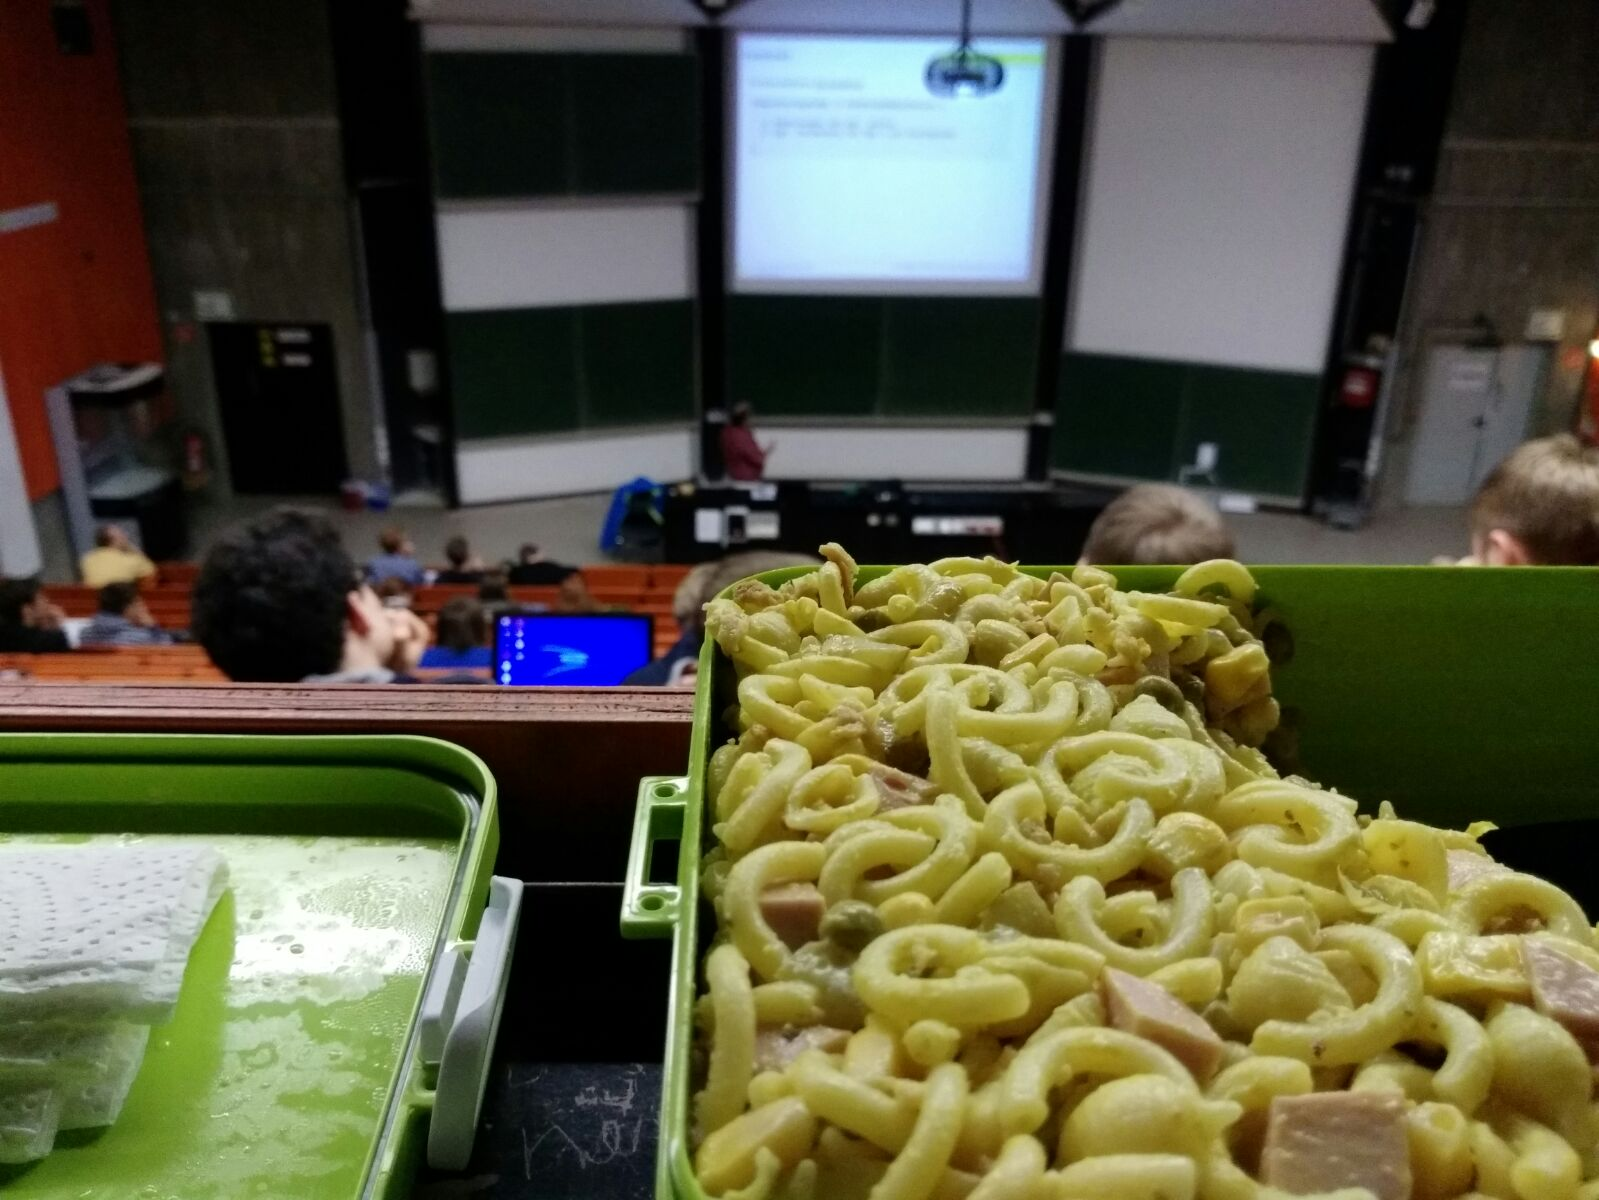
\includegraphics[width=.5\textwidth]{lasse/Nudelsalat.jpeg}
\end{figure}

\begin{recipe}
    [ % Optionale Eingaben
        preparationtime = {\unit[40]{min}},
        portion = \portion{6-10},
        %calory,
        source = Lasse
    ]
    {DER Nudelsalat}
    
    \introduction{
        \# orgasmischlecker
    }
    

    \ingredients
    {% Zutatenliste
        \unit[500]{g} & Suppennudeln \\
        \unit[1]{Dose} & Mais \\
        \unit[1]{Dose} & Erbsen \\
        \unit[1]{Gl} & Gewürzgurken \\
        \unit[1]{}  & Kleine Fleischwurst \\
         & Majo \\
         & Röstzwiebeln \\
        Gewürze & Pfeffer, Salz, Curry
    }
    
    \preparation
    { % Schrittweise Zubereitung
        \\
        Die Nudeln in Salzwasser nach Anleitung al Dente kochen und abkühlen lassen oder mit kaltem Wasser abspülen.
        
        Mais und Erbsen abtropfen lassen und die Gurken (gegebenenfalls auch die FLeischwurst) in ähnlich große Stücke schneiden.
        
        Alles in eine große Schüssel geben und verrühren. Drei bis vier große aufgehäufte Löffel Majonese mit verrühren. Mit Salz und Pfeffer und ORDENTLICH Curry würzen, bis keine Majofarbigen Flecken verbleiben.
        
        Röstzwiebeln am besten frisch auf dem Teller dazu nehmen. 
        
    }
    
    \hint
        {% Hinweise
        Nudeln können persönlich optimiert werden, ich empfehle 50/50 Eiermuscheln und Gabelspaghetti für die perfekte Löffelkonsistenz. 
        
        Natürlich auch ohne Fleischwurst möglich und vegane Remoulade o.Ä. ersetzen gut die Majo. (Wunderschlag wirkt Wunder). 
        
        Das Bild wurde von einem fleißigen Koch generiert.
        }
    
    \end{recipe}
    
\newpage
\begin{figure}
    \centering
    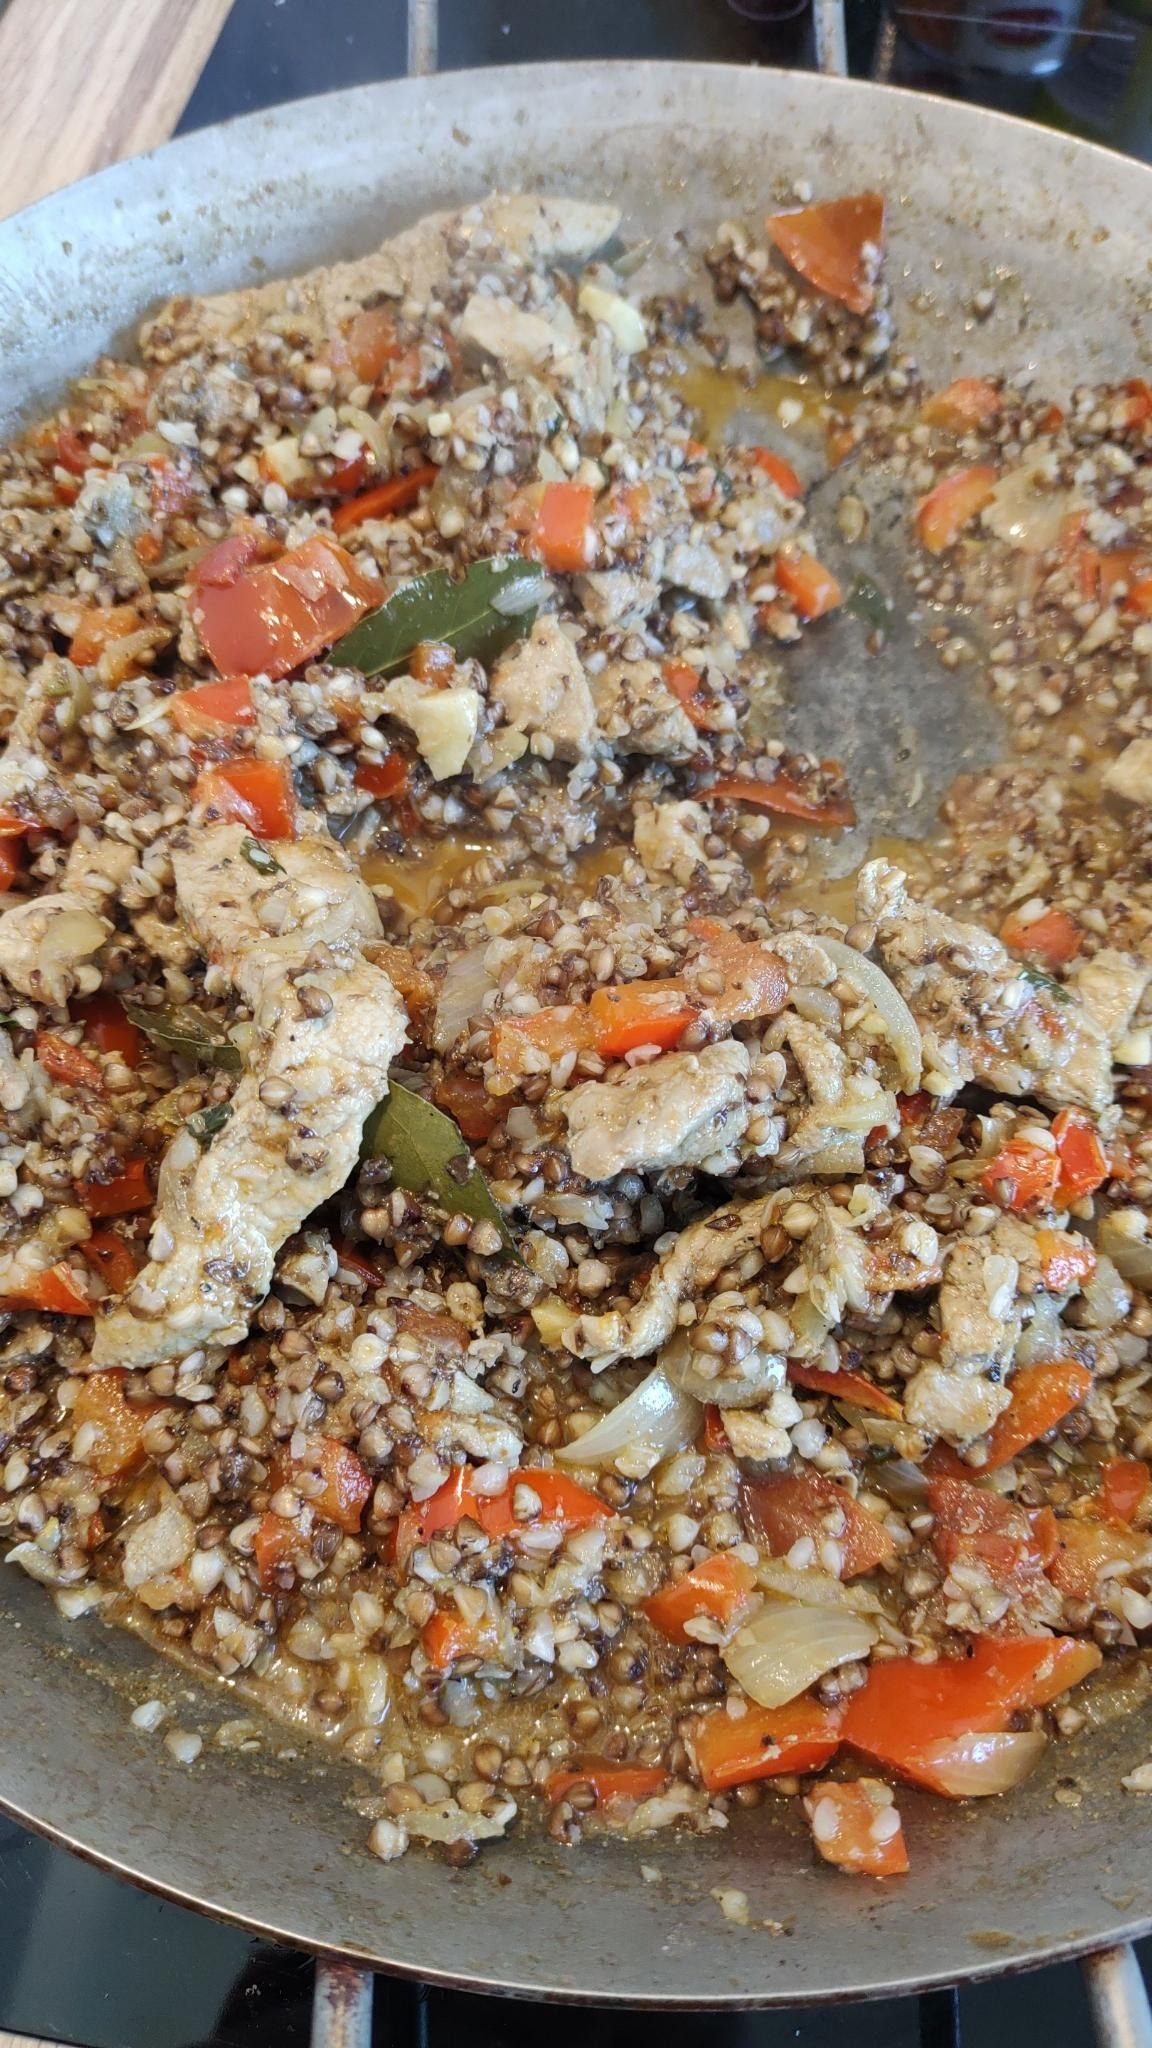
\includegraphics[angle=90, width=.5\textwidth]{lasse/Buchweizenpfanne.jpeg}
\end{figure}
\begin{recipe}
    [ % Optionale Eingaben
        preparationtime = {\unit[45]{min}},
        portion = \portion{3-4},
        %calory,
        source = Lasse
    ]
    {Leckere Pfanne}
    
    \introduction{
        \# Resteverwertstoffhof
    }
    

    \ingredients
    {% Zutatenliste
        \unit[500]{g} & Geschnetzeltes Geflügel \\
        \unit[1]{Tasse} & Buchweizen \\
        \unit[2.5]{Tassen} & Wasser \\
        1 & Paprika \\
        2 & Große Tomaten \\
        2 & Zwiebeln \\
        Wohlfühl & Knoblauch \\ 
        Gewürze & Pfeffer, Salz, Curry, Paprika
    }
    
    \preparation
    { % Schrittweise Zubereitung
        \\
        Die Zwiebeln schälen und schön klein schneiden. Die Paprika und die Tomaten waschen und in kleine Quadrate schneiden. Die gewünschte Menge Knoblauch vorbereiten.
        
        Das Fleisch mit den Zwiebeln anbraten. Sobald das Fleisch durch ist die Paprika und die Tomaten mit dem Knoblauch hinzugeben, nochmal zehn minuten unter geschlossenem Deckel im eigenen Saft braten. Hier mit Curry, Salz, Pfeffer würzen und ein Lorbeerblatt hinzugeben. 
        Den Buchweizen kurz auswaschen.
        
        Das Wasser in die Pfanne geben und den Buchweizen unterrühren. Die Hitze der Pfanne hoch drehen, dass das Wasser schnell wieder kocht. Solange offen köcheln, bis der Buchweizen sämtliches Wasser aufgenommen hat, dabei ab und zu über den Boden rühren.\hspace{5mm}Feddich :D
        
    }
    
    \hint
        {% Hinweise
        Schmeckt sehr gut auch mit einem Löffelchen Schmand im Teller. 
        
        Zusätzlich zur Paprika bietet sich eigentlich jegliches Gemüses und Konsorten an, die gerade weg müssen. Und geht natürlich auch alles ohne Fleisch, dann tut aber ein bisschen Butter oder Margarine gut. 
        
        Das Bild wurde von einem glücklichen Koch generiert.
        }
    
    \end{recipe}
    
\newpage

\begin{figure}
	\centering
	
\includegraphics[width=.25\textwidth]{lasse/oreo_curd.jpg}\hspace{3mm}
	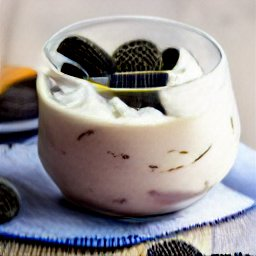
\includegraphics[width=.25\textwidth]{lasse/oreo_curd1.jpg}\hspace{3mm}
	
\includegraphics[width=.25\textwidth]{lasse/oreo_curd2.jpg}\hspace{3mm}
\end{figure}
    



\begin{recipe}
    [ % Optionale Eingaben
        preparationtime = {\unit[50]{min}},
        portion = \portion{6},
        %calory,
        source = Lasse (Malin)
    ]
    {Oreo Quark}
    
    \introduction{
        \# Kalorienbombe EXTREM
    }
    

    \ingredients
    {% Zutatenliste
        \unit[2]{Pkg} & Oreo Kekse \\
        \unit[250]{g} & Quark \\
        \unit[75]{g} & Puderzucker \\
        \unit[100]{g} & Frischkäse \\
        \unit[300]{ml} & Sahne \\
        \unit[2]{Pkg} & Paradiescreme Vanille 
    }
    
    \preparation
    { % Schrittweise Zubereitung
        \\
        Die Kekse 1 Tag vor der Zubereitung einfrieren. Die gefrorenen Kekse mit einer Keule je nach Geschmack fein oder grob zerdeppern.

        Quark, Puderzucker und Frischkäse gut verrühren. Die Sahne schlagen. Die Paradiescreme nach Packungsanleitung anrühren. Die Quarkmischung mit Paradiescreme verrühren und die Sahne unterheben.

        Nun abwechselnd die Creme mit den gemahlenen Keksen in eine Glasschüssel schichten, dabei mit einer Cremeschicht anfangen und mit einer Keksschicht aufhören.
    }
    
    \hint
        {% Hinweise
        Sollte man am besten kalt essen. Also eventuell nochmal eine Runde in den Kühlfrank. 
        
        Die Oreos müssen nicht unbedingt gefroren sein, das macht es nur leichter. 
        
        Die Bilder wurden von einer glücklichen KI generiert.
        }
    
    \end{recipe}
    
\newpage
% Aleksandra
\begin{figure}
    \centering
    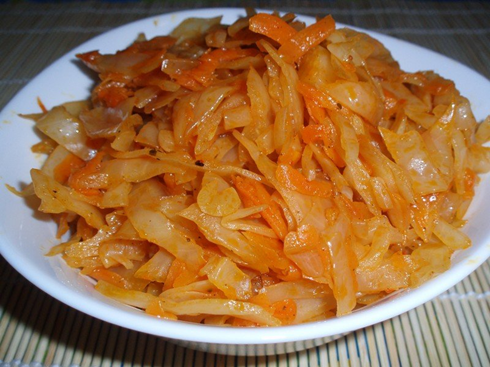
\includegraphics[width=.5\textwidth]{aleksandra/kapusta.png}
\end{figure}

\begin{recipe}
    [ % Optionale Eingaben
        preparationtime = {50 min},
        portion = sehr viel,
        source = Aleksandra
    ]
    {Schmorkohl}

\introduction{
    \# Schmeckt besser als er aussieht
}

\ingredients
{% Zutatenliste
    \unit[1]{} & Kohlkopf \\
    \unit[500]{g} & Sauerkraut \\
    \unit[2]{} & Zwiebeln \\
    \unit[1-2]{} & Möhren   \\    
    \unit[500]{g} & passierte Tomaten \\        
    \unit[2]{} & Zwiebeln \\
     &  Öl       \\
     & Pfeffer \\
    mögl. & Lorbeerblatt \\
    mögl. & Schinkenwürfel / Cranberries \\
}


\preparation
{ % Schrittweise Zubereitung
    \\
    Zwiebel, Möhre schälen, würfeln; Kohl in dünne (etwa Stiftdicke) und längliche (Fingerlang) Streifen schneiden.
    Zwiebeln, Möhren (ggf Schinkenwürfel) im Topf andünsten lassen bis die Zwiebeln glasig werden. \\
    
    Sauerkraut, Kohl in den Topf geben, mit Tomatenmark übergießen, versuchen, umzurühren.\\ 
    
    Etwas Salz, viel Pfeffer dazugeben (ungewöhnlich große Menge, da ungewöhnlich viel Kohl). Die Lorbeerblätter 5-10 Minuten vor Ende dazugeben.
    Schmoren lassen. Der Kohl ist fertig, wenn er zwar nicht mehr knackig ist, aber auch nicht gänzlich labberig. \\
    
    Den Schmorkohl kann man gut als Beilage zu allem essen. Er schmeckt auch kalt. Wenn ich crazy drauf bin, esse ich ihn mit einem Löffel Schmand.    }



\hint
{% Hinweise
    Nimm den größeren Topf.         
}


\end{recipe}

\newpage
\begin{figure}
    \centering
    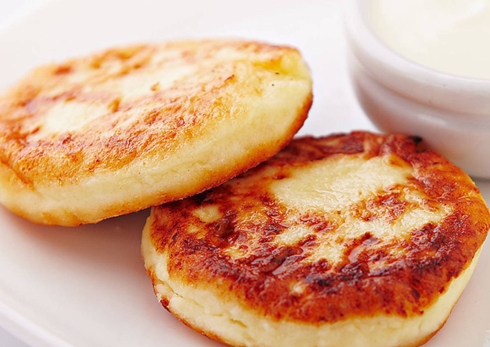
\includegraphics[width=.35\textwidth]{aleksandra/sirnik.png}
\end{figure}

\begin{recipe}
    [ % Optionale Eingaben
        preparationtime = {\unit[max. 45]{min}},
        portion = für drei Personen und es bleibt noch ein wenig übrig für Morgen,
        source = Aleksandra
    ]
    {Sirniki}

    \introduction{
        \# die beste Gesellschaft für Tee
    }


\ingredients
{% Zutatenliste
    \unit[500]{g} & Quark (möglichst trocken)\\
    \unit[1-2]{} & Eier \\
    \unit[2-4]{EL} & Zucker \\
    \unit[3-5]{EL} & Mehl \\
     & Sonnenblumen-/Rapsöl \\
    mögl. & Backpulver \\
    mögl. & Rosinen/ \\
    & Cranberries/ \\
    & Apfelstücke
}

\preparation
{ % Schrittweise Zubereitung
\\
Achtung, damit der Teig zusammenpappt und nicht auseinanderläuft muss er möglichst viel Flüssigkeit verlieren. Dafür muss er min. 24\,h abtropfen. Dazu kann er in einem Sieb oder einem Stück Mull über der Spüle aufgehangen werden. Vor der Zubereitung kann man das Paket nochmal quetschen.

Alle Zutaten in einer Schüssel miteinander verkneten, bis eine Masse entsteht, die die Konsistenz von weicher Knete oder Kartoffelpüree ähnelt.

Daraus Kreise kneten, die etwa handflächengroß und daumendick oder dicker sind. 
In der Pfanne von beiden Seiten goldbraun werden lassen. Je nach Pfanne und Hitzestufe braucht jeder Sirnik 2-5 Minuten.

Essen kann man Sirniki pur, mit Schmand, Honig oder Marmelade zu einer heißen Tasse Tee. Sie schmecken auch kalt gut.
}

\hint
{% Hinweise
Um die einzelnen Sirniki zu formen hilft es, wenn die Hand angemehlt ist. Dann erst Kugeln formen und sie anschließend zerdrücken.\\ 
Am schnellsten (aber auch stressigsten) geht es, die Pfanne zu erhitzen, bis das Öl heiß wird, die ersten Sirniki vorzubereiten und braten, sobald das Öl heiß ist. Während sie brutzeln, kann man dann die nächsten vorbereiten. \\
Viel Öl hilft viel. \\
Einen Teller bereithalten, um die fertigen Sirniki abzulegen. Um das Pfannenfett einzusaugen, kann man auf den Teller ein Papiertuch legen.        
}

    \end{recipe}

\newpage
\begin{recipe}
    [ % Optionale Eingaben
        preparationtime = {\unit[50]{min}},
        portion = Ein Topfvoll,
        source = Aleksandra
    ]
    { Mußacha }

\introduction{
    \# Herzhafte GeSCHICHTEN
}


\ingredients
{% Zutatenliste
    & \textbf{egal, wie viel. Hauptsache von allem ungefähr gleich}  \\
    \unit[]{} & Tomate \\
    \unit[]{} & Aubergine \\
    \unit[]{} & Kartoffel \\
    \unit[]{} & Hackfleisch \\       
    \unit[]{} & ggf Paprika \\
    \textbf{viel} & Gewürze: Pfeffer, Knoblauch, Lorbeer, Thymian, Rosmarin,..  
}

\preparation
{ % Schrittweise Zubereitung
\\
Alle Zutaten in maximal CD-Hüllen dicke Kreisscheiben schneiden, außer die Zwiebeln. Die würfelst du.

Diese richtest du Schichtweise in einem relativ hohen Topf an, sodass jede Schicht mindestens zwei Mal vorkommt. Füll den Topf min zu einem Viertel mit Wasser.

Auf mittlerer bis höherer Hitze mit Deckel köcheln lassen bis alle Schichten durch sind.

Heiß essen, wenn du willst mit Schmand und mit ein Paar Stängeln Petersilie.
}

\hint
    {% Warnhinweis
    Achtung! Sehr lecker.
    }

\end{recipe}

\newpage

% Eva
\begin{recipe}
[ % Optionale Eingaben
    preparationtime = {\unit[10-80]{min}, abhängig von der Ofenqualität und Menge},
    %bakingtime={\unit[6]{h}},
    %bakingtemperature={\Fanoven\ \unit[170]{C}},
    %portion = \portion{8},
    %calory,
    source = Eva
]
{Pfannkuchen}

\introduction{
    \# Das einzige Rezept, das ich kann
}

\graph{
    small = eva/pfannkuchen_durchschnittlich, %offensichtliches Bild auf dem Desktop 1,
    big = eva/pfannkuchen_fancy %offensichtliches Bild auf dem Desktop 2,
}

\ingredients
{% Zutatenliste
    \unit[\nicefrac{1}{2}]{Einheit} & Mehl, z.B. \unit[500]{g} \\
    \unit[1]{Einheit} & Milch, z.B. \unit[1]{l} \\
    \unit[1] & Ei \\
    wenig & Backpulver \\
    genug & Zimt \\
    beliebiger & Belag \\
}

\preparation
{ % Schrittweise Zubereitung
    \\
    Man nehme doppelt so viel Milch wie Mehl und ein Ei pro \unit[500]{g} Mehl. Oder einfach immer ein Ei.
    Oder so viele, wie man grade da hat und loswerden möchte. Und mische es zusammen.

    Gute Ergänzungen sind etwas Backpulver oder Zimt. Auch davon kann jeweils beliebig viel hinzugefügt werden.
    Es empfiehlt sich ungefähr eine Prise Backpulver und eine Schüsseloberfläche voll Zimt. Evtl. kann auch eine Prise
    Salz hinzugefügt werden.

    Anschließend mischt man alles gut mit einem Schneebesen oder Rührgerät durch - es kann auch erst lange 
    umgerührt, dann der Zimt hinzugefügt und dann nochmal kurz umgerührt werden - und erhitzt den Teig passend zur 
    zur Verfügung stehenden Pfanne portioniert in einer Pfanne.
}

\hint
    {% Hinweise
    Erinnerst du dich, dass wir uns irgendwann darüber unterhielten, welches Essen dasjenige sei,
    von dem man sich im Zweifelsfall am ehesten ausschließlich ernähren könnte? Ich glaube, Brot wäre gut. Aber solltest
    du dich doch mal gegen Suppe entscheiden, hast du jetzt dieses nützliche Rezept :)
    
    Der Belag ist wirklich sehr frei wählbar. Ich nehme oft Apfelmus mit mehr Zimt, oder nichts oder Marmelade. Frevlerische 
    Individuen mögen aber beispielsweise auch die Kombination Tomate und Käse.
    }

\end{recipe}

\newpage


\end{document}
